\documentclass{article}
\usepackage[utf8]{inputenc}
%%%%%%%%%%%%%%%%%%%%%%%%%%%%%%
% Preámbulo
%%%% Escritura en español 

\usepackage[T1]{fontenc}
\usepackage[utf8]{inputenc}
\usepackage[spanish, es-tabla]{babel}
%%%% Espacio entre párrafos y cajas de texto con \mbox y \fbox
\usepackage{parskip}
\usepackage{amsmath}
\usepackage{physics}
\usepackage{subcaption}
%%%% Modificar tamaño de sangría
\setlength{\parindent}{0.5in}
%%%%%colores de letra, color de fondo, borde.
\usepackage[usenames, dvipsnames]{xcolor}
%%%% Definir un nuevo color
\definecolor{cafe}{RGB}{93,36,23}
\definecolor{Verde}{RGB}{0,187,45}
%%%% Expresiones matemáticas 
\usepackage{amsmath}
\usepackage{amssymb,amsfonts,latexsym,cancel,mathrsfs}
%%%% Jerarquía numeración de ecuaciones, figuras y tablas
\usepackage{enumitem}
\numberwithin{equation}{section}
\numberwithin{figure}{section}
\numberwithin{table}{section}
%%%% Gráficas
\usepackage{graphicx}
%%%% Ubicar dos imágenes juntas
\usepackage{caption}
\usepackage{subcaption}
%%%% Poner varias figuras en \figure 
%\usepackage{subfigure}
%%%% Convertir figuras de formato eps pdf
\usepackage{epstopdf}
%%%% Ubicación de una gráfica o tabla
\usepackage{float}
%%%% Formato a las tablas
\usepackage{array}
\usepackage{longtable}
%%%% Crear lista con varias columnas
\usepackage{multicol}
\usepackage{multirow}
%%%% Entorno matemático en las tablas
\newcolumntype{E}{>{$}c<{$}}
\newcolumntype{L}{>{$}l<{$}}
\newcolumntype{R}{>{$}r<{$}}
%%%% Imagen en medio del texto
\usepackage{wrapfig}
%%%% Negrilla en modo matemático
%\usepackage{bm}
%%%% Referencias .bib (para citar \cite{•)}
%\usepackage[backend=biber]{biblatex}
%\usepackage[style=apa, backend=biber]{biblatex}
\usepackage[spanish]{babel} % o el idioma que estés usando
\usepackage{csquotes} % Agrega esta línea para cargar csquotes
\usepackage[usenames]{color}
\renewcommand{\theequation}{\arabic{equation}}
%--------------------------------------------------
%Para agregar citas en apa
%Para citar se usa el comando \cite{}
%Las referencias se modifican en el archivo sample.bib
%\lef\cite\shortcite{}
%\usepackage{apacite}
%----------------------------------------------




\usepackage[maxbibnames=99, sorting=none, backend=bibtex]{biblatex}
\addbibresource{ref.bib}

\usepackage{setspace} %para el interlineado

\setlength{\parindent}{0cm} %sangria de los parrafos
\usepackage{comment}

%%%%%%%%% Configuración de margenes
\usepackage[lmargin=0.5in,rmargin=0.5in,top=0.5in,bottom=0.5in]{geometry} %margen izquierdo, margen derecho, encabezado, parte inferior 
%%%%Formato zona superior
%\usepackage{fancyhdr}
%\pagestyle{fancy}
% Modificaciones
%\fancyhead{} % Eliminamos definiciones previas de la zona superior 
%\fancyhead[L]{\emph{\textbf{Materia} Titulo del documento}} %Posición, tamaño de texto y texto 

%\fancyhead[R]{\includegraphics[scale=0.13]{Imagenes/Escudo Udenar.png} }%Posición, imagen 

%\fancyfoot{} % Eliminamos definiciones previas de la zona inferior
%\fancyfoot[C]{\thepage} %Posición, número de pagina 

%\fancyfoot[L]{Christian Martínez} %Posición, Texto
%\renewcommand{\headrulewidth}{0.5pt} %Grosor de la línea superior
%\renewcommand{\footrulewidth}{0.5pt} %Grosor de la línea inferior
%\renewcommand{\baselinestretch}{1.5}
 
%%%%%%% Portada
\begin{document}
\begin{center}
    \textbf{UNIVERSIDAD NACIONAL DE COLOMBIA} \\
    \vspace{0.2cm}
    \small{Facultad de Ciencias - Departamento de Física} \\
    \vspace{0.2cm}
    \small{Dosimetría} \\
    \vspace{0.5cm}
    \large{\textbf{Determinación de niveles de referencia de dosis}} \\
    \vspace{0.2cm}
    
    \vspace{0.5cm}
    \small{Oscar Andrés Azula Chaves } \\
    \vspace{0.2cm}
    \small{\today} \\
    \vspace{0.5cm}
    \rule{\textwidth}{0.5pt} \\
    \vspace{1cm}
\end{center}







\section{Introducción}

Este informe presenta la evaluación de Niveles de Referencia Diagnósticos (DRL) de radiología convencional y tomografía computada a partir de datos locales de práctica clínica del HUN desde Julio a Septiembre del 2025. Se analizaron las métricas dosimétricas disponibles ( Dosis Total [mGy], Dosis [mGy] por proyección, CTDIvol y DLP en TC), agrupadas por procedimiento y, cuando aplica, por proyección y por rangos de peso del paciente. La estimación de DRL se basa en el percentil 75 (P75) de las distribuciones por procedimiento, de acuerdo con las recomendaciones internacionales (ICRP 135). Los resultados permiten comparar la práctica local con valores de referencia externos y priorizar acciones de optimización.

El proceso DRL debe utilizarse para evaluar si, en circunstancias habituales,
la cantidad de radiación ionizante aplicada en un procedimiento de diagnóstico por imagen en
un centro sanitario local, cuando se evalúa para una muestra representativa de pacientes (no
pacientes individuales) para una tarea clínica definida, es demasiado alta o demasiado baja.

\section{Radiología convencional}



Para radiología convencional se restringio el calculo a los procedimientos cuya frecuancia fuera mayor al 28, de los 41 estudios que se tenian se restringió a los procedimientos de Tórax, Pelvis, Rodilla, Mano, Abdomen, Lumbar, Hombro y Pie(figura \ref{fig:cant_r}).
\begin{figure}[h]
    \centering
    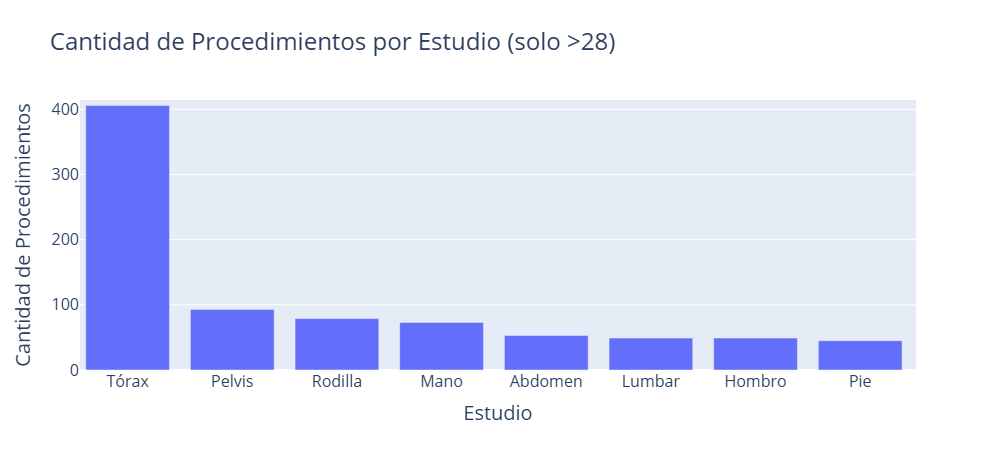
\includegraphics[width=0.8\linewidth]{cantodad_estudios.png}
    \caption{Frecuencia de estudios de radiología convencional según región anatómica. Los datos estudiados abarcan desde Junio hasta Septiembre y se limito a los procedimientos con una frecuencia mayor a 28.}
    \label{fig:cant_r}
\end{figure}


Para estos estudios se realizaron 2 boxplot, el primero para los procedimientos ubicados en el tronco (figura \ref{fig:upper}) y otro para extremidades (figura \ref{fig:extremidades}). Acorde a lo esperado se evidencia que para los procedimientos de extremidades la dosis total es considerablemente menor a comparación de abdomen, pelvis y tórax. La presencia de asimetría y valores atípicos conlleva a que el promedio (linea discontinua) sea en todos los casos mayor a la mediana. 



\begin{figure}[h]
    \centering
    \begin{minipage}{0.48\linewidth}
        \centering
        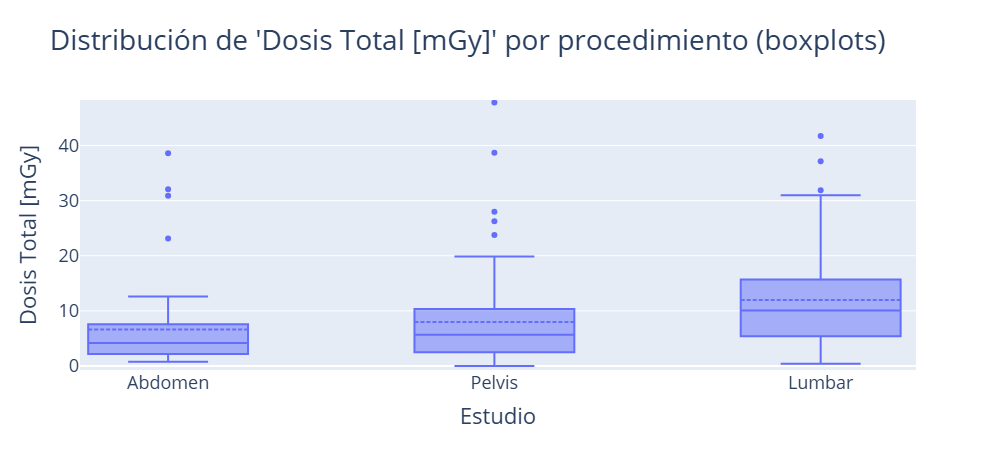
\includegraphics[width=\linewidth]{Graficas/boxes_upper.png}
        \caption{Boxplot de los procedimientos seleccionados ubicados en el tronco.}
        \label{fig:upper}
    \end{minipage}
    \hfill
    \begin{minipage}{0.48\linewidth}
        \centering
        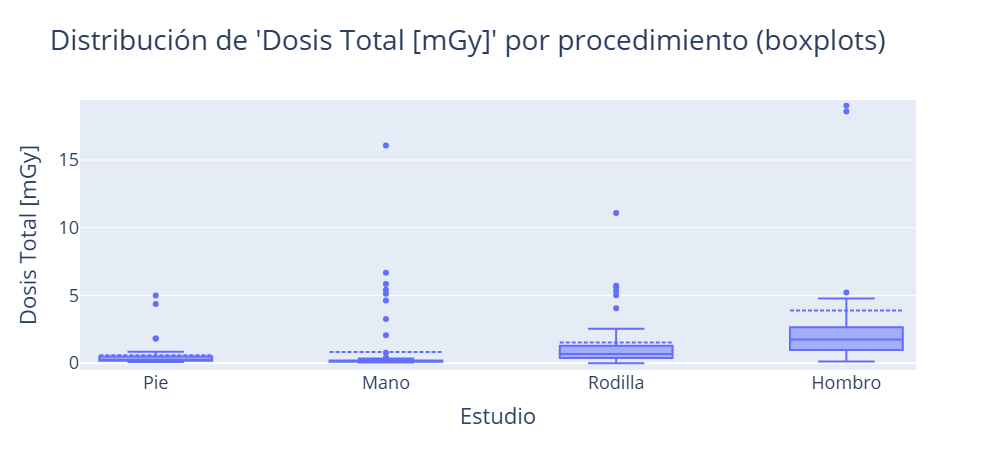
\includegraphics[width=\linewidth]{Graficas/boxes_extremidades.png}
        \caption{Boxplot de los procedimientos seleccionados correspondientes a extremidades anatómicas.}
        \label{fig:extremidades}
    \end{minipage}
\end{figure}

Ademas de la dosis total también se tiene la dosis por proyección para cada procedimiento (figura \ref{fig:proyect}) en los cuales los procedimientos de abdomen, pelvis y lumbar presentan los promedios de dosis más elevados, coherente con el mayor espesor de tejido a atravesar y la necesidad de penetración ósea. 
\begin{figure}[h]
    \centering
    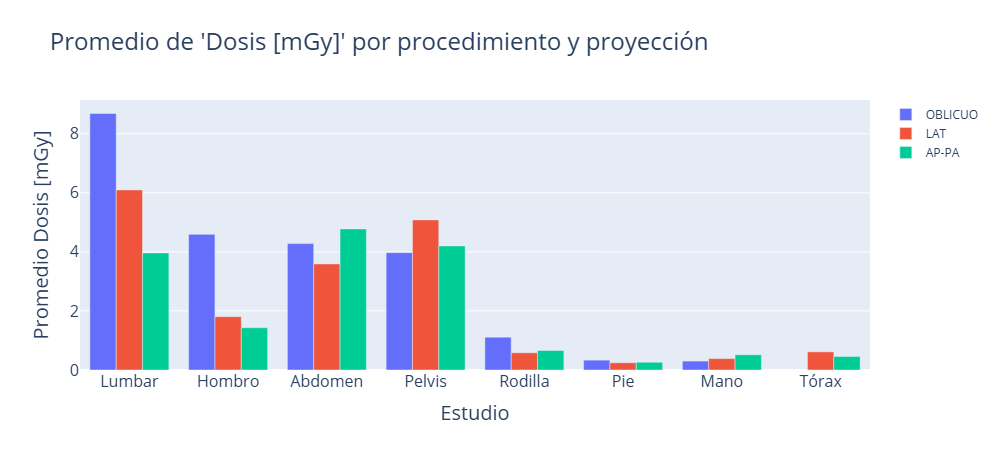
\includegraphics[width=0.8\linewidth]{Graficas/promedio_dosis_por_proc_proyec.png}
    \caption{Diagrama de barras agrupadas  que muestra el promedio de dosis de radiación (en $mGy$) para diferentes procedimientos (Estudio) y proyecciones radiográficas (Proyección). Cada grupo en el eje X corresponde a un tipo de estudio, y dentro de cada grupo hay una barra para cada proyección asociada. La altura de cada barra representa el valor promedio de la dosis registrada para ese estudio y proyección.}
    \label{fig:proyect}
\end{figure}


Analizando la dosis promedio para rangos de peso desde 50[kg] a 90[kg] se resisaron las gráficas de la figura \ref{fig:panel_hist}. Muestran la relación entre el peso del paciente y la dosis promedio administrada para cada tipo de estudio radiográfico. Se observa que para la mayoría de procedimientos existe una tendencia creciente de la dosis con el aumento del peso, lo cual es esperado debido a la mayor atenuación de los rayos X en pacientes con mayor masa corporal

\begin{figure}[H]
    \centering
    \begin{subfigure}[b]{0.45\linewidth}
        \centering
        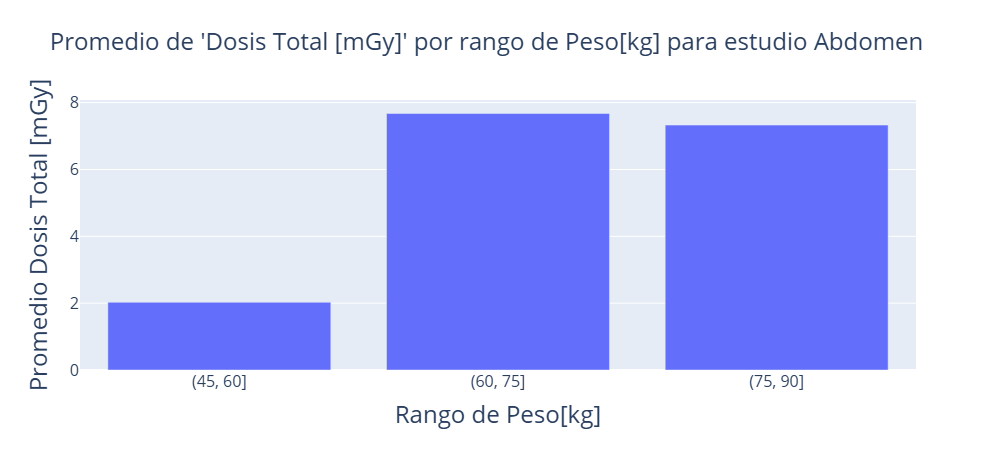
\includegraphics[width=\linewidth]{Graficas/abdomen_hist.png}
        \caption{}
        \label{fig:abdomen}
    \end{subfigure}
    \begin{subfigure}[b]{0.45\linewidth}
        \centering
        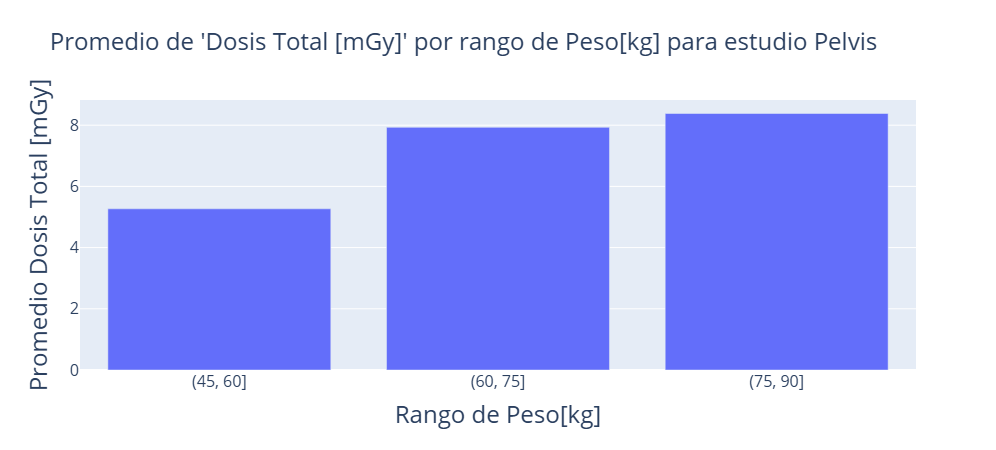
\includegraphics[width=\linewidth]{Graficas/pelvis.png}
        \caption{}
        \label{fig:pelvis}
    \end{subfigure}
    
    \begin{subfigure}[b]{0.45\linewidth}
        \centering
        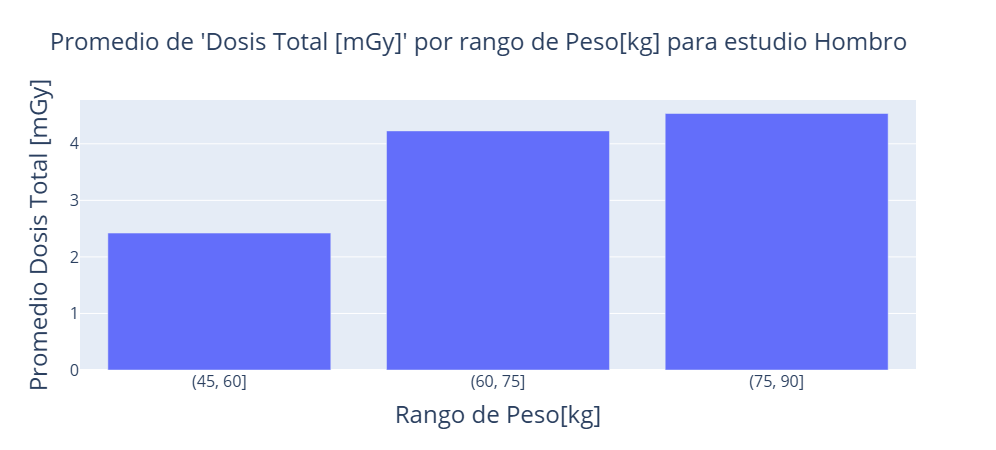
\includegraphics[width=\linewidth]{Graficas/hombro.png}
        \caption{}
        \label{fig:hombro}
    \end{subfigure}
    \begin{subfigure}[b]{0.45\linewidth}
        \centering
        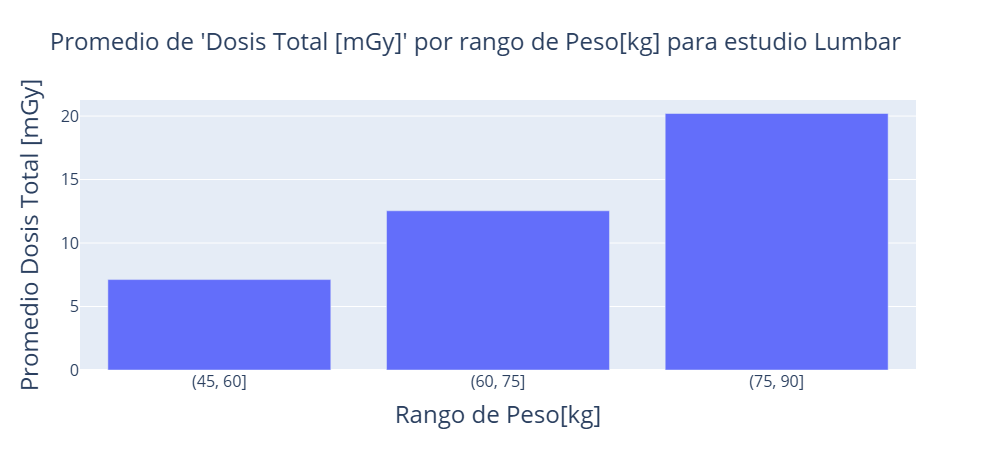
\includegraphics[width=\linewidth]{Graficas/lumbar.png}
        \caption{}
        \label{fig:lumbar}
    \end{subfigure}
    
    \begin{subfigure}[b]{0.45\linewidth}
        \centering
        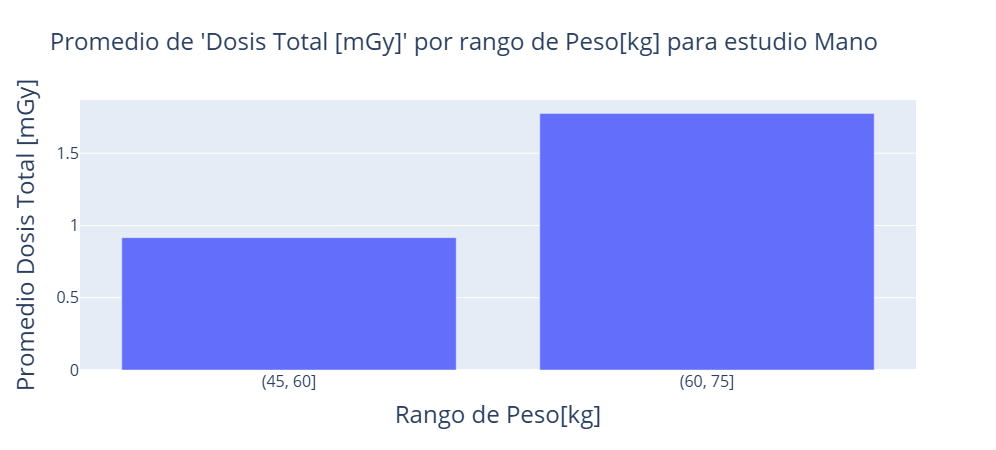
\includegraphics[width=\linewidth]{Graficas/mano.png}
        \caption{}
        \label{fig:mano}
    \end{subfigure}
    \begin{subfigure}[b]{0.45\linewidth}
        \centering
        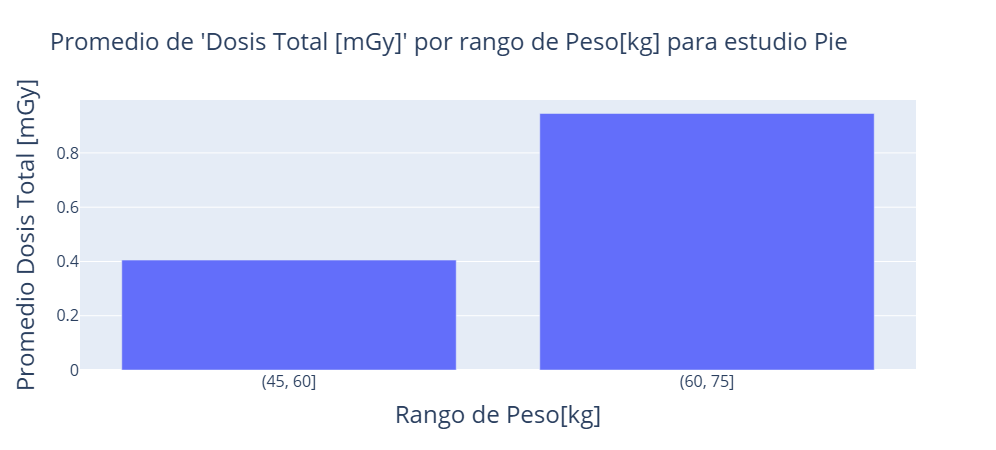
\includegraphics[width=\linewidth]{Graficas/pie.png}
        \caption{}
        \label{fig:pie}
    \end{subfigure}
    
    \begin{subfigure}[b]{0.45\linewidth}
        \centering
        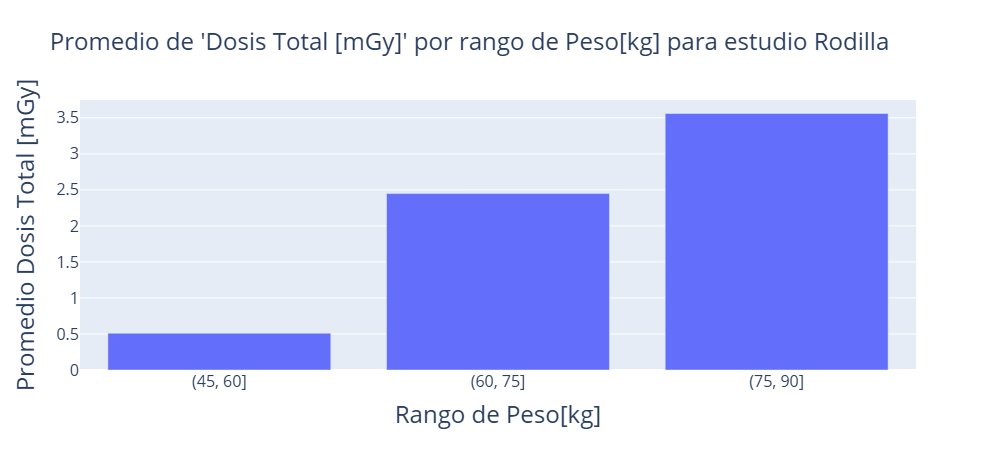
\includegraphics[width=\linewidth]{Graficas/rodilla.png}
        \caption{}
        \label{fig:rodilla}
    \end{subfigure}
    \begin{subfigure}[b]{0.45\linewidth}
        \centering
        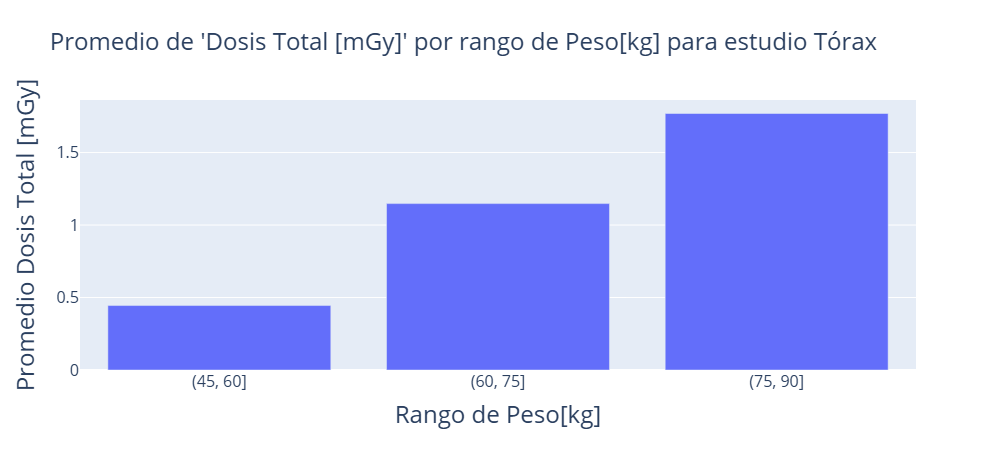
\includegraphics[width=\linewidth]{Graficas/torax.png}
        \caption{}
        \label{fig:torax}
    \end{subfigure}

    \caption{Promedio de la dosis total en el rango de peso de 50 a 90 kg, considerando 9 procedimientos de diferentes regiones anatómicas en radiología convencional: (a) Abdomen, (b) Pelvis, (c) Hombro, (d) Lumbar, (e) Mano, (f) Pie, (g) Rodilla, (h) Tórax. La dosis total es la suma de la dosis por proyección.}
    \label{fig:panel_hist}
\end{figure}


\begin{table}[h]
\centering
\caption{Promedio de dosis total por rango de peso corporal y tipo de procedimiento radiográfico}
\label{tab:dosis_peso}
\begin{tabular}{|c||c|c|c|c|c|c|c|c|} 
\hline
\textbf{Rango de Peso (kg)} & \textbf{Abdomen} & \textbf{Hombro} & \textbf{Lumbar} & \textbf{Mano} & \textbf{Pelvis} & \textbf{Pie} & \textbf{Rodilla} & \textbf{Tórax} \\ \hline
45-60 & 2.03 (7) & 2.42 (8) & 7.12 (12) & 0.92 (7) & 5.27 (11) & 0.41 (8) & 0.51 (15) & 0.44 (64) \\ \hline
60-75 & 7.68 (31) & 4.23 (33) & 12.54 (24) & 1.77 (13) & 7.93 (30) & 0.95 (15) & 2.45 (31) & 1.15 (168) \\ \hline
75-90 & 7.33 (7) & 4.54 (7) & 20.20 (7) & -- & 8.38 (15) & -- & 3.56 (4) & 1.77 (36) \\ \hline
\end{tabular}
\begin{minipage}{\textwidth}
\footnotesize
\textbf{Nota:} Los valores se presentan como promedio de dosis (mGy) con el número de procedimientos entre paréntesis. Los guiones (--) indican rangos sin datos.
\end{minipage}
\end{table}



\section{Tomografía}

Para tomografia computada se restringio el calculo a los procedimientos cuya frecuancia fuera mayor a 170 como se evidencia en la grafica \ref{fig:cant_tomo}.

\begin{figure}[h]
    \centering
    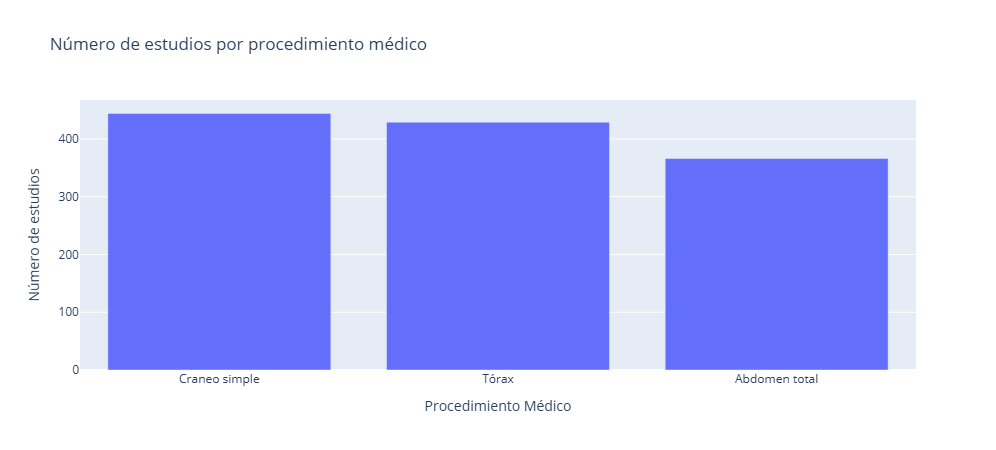
\includegraphics[width=0.8\linewidth]{Graficas/cantidad_tomo.png}

        \caption{diagrama de barras (bar chart) que muestra la cantidad de estudios realizados para cada tipo de procedimiento médico de tomografía.}
    \label{fig:cant_tomo}
\end{figure}

Con los valores de DLP y CTDI_{vol} se realizo el promedio para los procedimientos de tomografía axial computada de cráneo simple, abdomen total y tórax en las figuras \ref{fig:dlp} y \ref{ctdi}.
\begin{figure}[h]
    \centering
    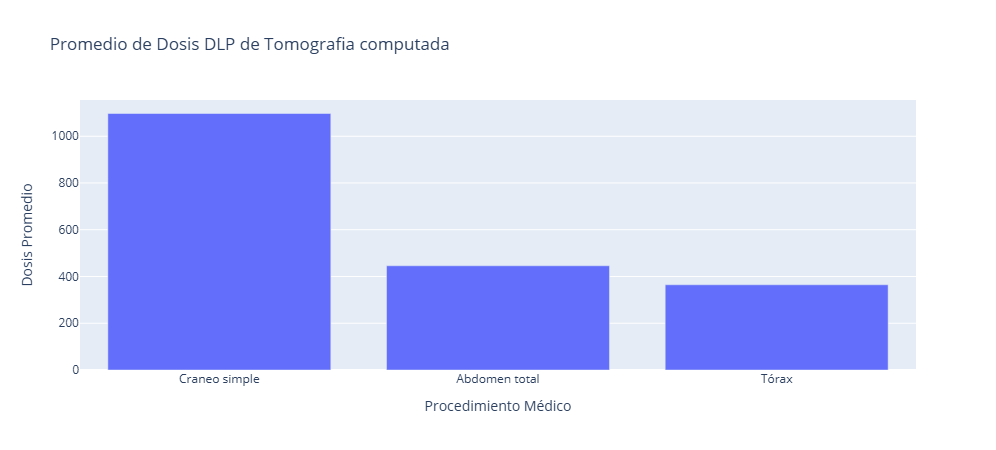
\includegraphics[width=0.8\linewidth]{Graficas/dlp.png}

        \caption{Muestra el promedio de DLP (Dose Length Product) para cada tipo de procedimiento médico. En el eje X se presentan los procedimientos y en el eje Y el valor promedio de DLP registrado para cada uno.}
    \label{fig:dlp}
\end{figure}

\begin{figure}[h]
        \centering
        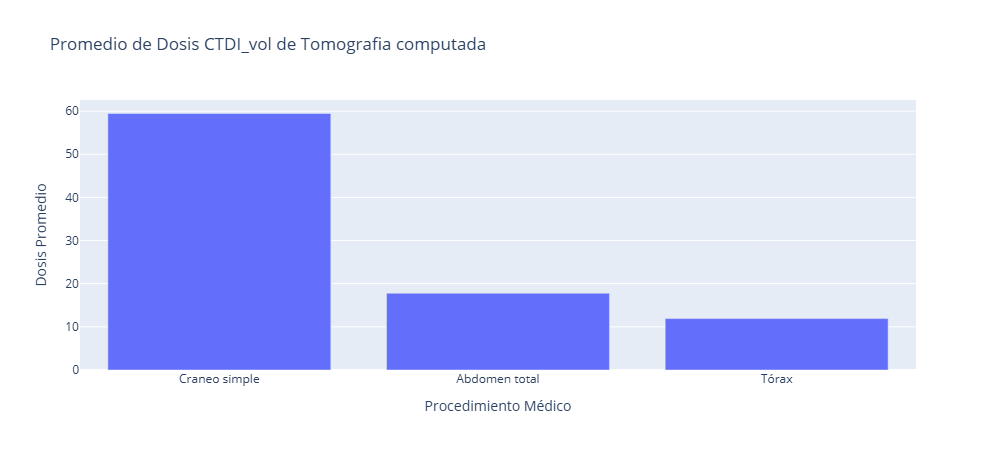
\includegraphics[width=0.8\linewidth]{Graficas/ctd.png}
        \caption{Muestra el promedio de CTDI vol (Computed Tomography Dose Index - volumen) para cada procedimiento. De nuevo, el eje X corresponde a los procedimientos y el eje Y al valor promedio de CTDI vol.}
        \label{ctdi}
    \end{figure}



\end{document}
